\documentclass[10pt,twocolumn]{article}
\usepackage[margin=0.75in]{geometry}                % See geometry.pdf to learn the layout options. There are lots.
\geometry{letterpaper}                   % ... or a4paper or a5paper or ... 
%\geometry{landscape}                % Activate for for rotated page geometry
%\usepackage[parfill]{parskip}    % Activate to begin paragraphs with an empty line rather than an indent
\setlength{\columnsep}{1cm}
\usepackage{graphicx}
\usepackage{amsmath}
\usepackage{amssymb}
\usepackage{epstopdf}
\usepackage{fullpage}
\usepackage[usenames]{color}
\usepackage{titlesec}
\usepackage{hyperref}
\usepackage{framed}

\definecolor{light-gray}{gray}{0.45}
\titleformat{\section}
{\color{black}\normalfont\huge\bfseries}
{\color{black}\thesection}{1em}{}

\titleformat{\subsection}
{\color{light-gray}\normalfont\Large\bfseries}
{\color{light-gray}\thesubsection}{1em}{}

\DeclareGraphicsRule{.tif}{png}{.png}{`convert #1 `dirname #1`/`basename #1 .tif`.png}

\title{\Huge{\bf Algorithm 1: Shapes}}
\author{Comp175: Computer Graphics -- Spring 2015}
\date{Due:  {\bf Wednesday Februrary 4th} at 11:59pm}                                           % Activate to display a given date or no date

\begin{document}
\maketitle
%\section{}
%\subsection{}

\begin{verbatim}
Your Names: Matt Brenman

            Matt Cardarelli

Your CS Logins: mbrenm01

                mcarda01\end{verbatim}

\section{Instructions}
Complete this assignment only with your teammate. You may use a
calculator or computer algebra system. All your answers should be given in simplest form.
When a numerical answer is required, provide a reduced fraction (i.e. 1/3) or at least three
decimal places (i.e. 0.333). Show all work; write your answers on this sheet. This algorithm handout is worth 3\% of your final grade for the class.


\section{Cube}
 {\bf [1 point]} Take a look at one face of the cube. Change the tessellation parameter. How do the number of small squares against one edge correspond to the tessellation parameter?
\vspace{2em}\\
The number of small squares against an edge is exactly the value of the tessellation parameter.
\vspace{2em} \\
{\bf [1 point]} Imagine a unit cube at the origin with tessellation parameter 2. Its front face lies in the +XY plane. What are the normal vectors that correspond with each of the eight triangles that make up this face? (Note: when asked for a normal, you should always give a normalized vector, meaning a vector of length one.)
\vspace{2em}\\
Each normal vector has the value $\begin{bmatrix} 0 \\ 0\\ 1 \end{bmatrix}$.
\vspace{2em}
\section{Cylinder}
{\bf [1.5 points]} The caps of the cylinder are regular polygons with $N$ sides, where $N$'s value is determined by parameter 2 ($p_2$). You will notice they are cut up like a pizza with $N$ slices, which are isosceles triangles. The vertices of the $N$-gon lie on a perfect circle. What is the equation of the circle that they lie on  in terms of the radius (0.5) and the angle $\theta$?
\vspace{2em}\\
Since the circlular caps are centered, we do not have to perform any transformations, so the equation for the caps are:

$r = 0.5$

\vspace{2em}
{\bf [1.5 points]} What is the surface normal of an arbitrary point along the barrel of the cylinder? It might be easier to think of this problem in cylindrical coordinates, and then transform your answer to cartesian after you have solved it in cylindrical coords.
\vspace{2em} \\
In cylindrical coordinates, the surface normal of an arbitrary point is: $\vec{v} = (1, \theta, 0)$. \\
In cartesian coordinates, this becomes $\vec{v} = (r*cos\theta, 0, r*sin\theta)$ and since $r = 1$ (as it is a unit vector), the final vector is $\vec{v} = (cos\theta, 0, sin\theta)$.
\vspace{2em}

\section{Cone}
{\bf [1 point]} Look at the cone with Y-axis rotation = 0 degrees, and X-axis rotation = 0 degrees. How many triangles make up one of the $segmentX$ ``sides'' of the cone when $segmentY=1$? When $segmentY=2$? 3? $n$? 
\begin{tabular}{c|c}
$segmentY$ & \# of triangles \\ \hline
1 & 1 \\
2 & 3 \\
3 & 5 \\
$n$ & $2n - 1$
\end{tabular}
\vspace{2em}\\
{\bf [1 point]} What is the surface normal at the tip of the cone? Keep in mind that a singularity does not have a normal; this implies that there will not be a unique normal at the tip of the cone. You can achieve a good shading effect by thinking of $segmentX$ vectors with their base at the tip of the cone, each pointing outward, normal from the face of the triangle assocated with it along the side of the cone. Think about how OpenGL can use this information to make a realistic point at the top of the cone, and draw a simple schematic sketch illustrating the normal for one of the triangles at the tip. (As long as it is clear that you get the idea, you will recieve full credit.)
\vspace{2em}\\
The surface normal of the tip of the cone should have as many normals as sides of the cone. Each would be parallel to the normals along the side of the cone. This would allow for the reflection of incoming light to not be affected by a linear interpolation by OpenGL and would allow for a more normal shading of the shape. The following image demonstrates this idea: \\
\begin{center}
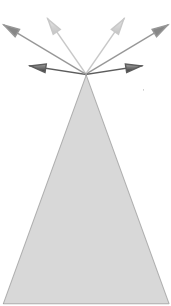
\includegraphics[width=8em]{graphicshw1cone} \\
\end{center}
\vspace{2em}
{\bf [1 point]} Take the two dimensional line formed by the points $(0, 0.5)$ and $(0.5, -0.5)$ and find its slope $m$.
\vspace{2em}
\begin{equation*}
m = \frac{\Delta x}{\Delta y} = \frac{-0.5 - 0.5}{0.5 - 0} = \frac{-1}{0.5} = -2
\end{equation*}
\vspace{2em}
{\bf [1 point]} ${{1}\over{m}}$ is the slope perpendicular to this line. Using this slope, we
can find the vertical and radial/horizontal components of the normal on the cone body. The radial/horizontal component is the component in the XZ plane. What is the {\bf magnitude} of this component in a normalized normal vector?
\vspace{2em}
\begin{equation*}
-\frac{1}{m} = -\frac{1}{-2} = \frac{1}{2} = \frac{v_y}{v_{xz}}\quad \ldots \quad
v_{xz} = \frac{2}{\sqrt{2^2 + 1^2}} = \frac{2}{\sqrt{5}}
\end{equation*}
\vspace{2em}\\
{\bf [1 point]} The componenet in the $y$ direction is the vertical component. What is the {\bf magnitude} of this component in a normalized normal vector?
\vspace{2em}
\begin{equation*}
-\frac{1}{m} = -\frac{1}{-2} = \frac{1}{2} = \frac{v_y}{v_x}\quad \ldots \quad
v_y = \frac{1}{\sqrt{2^2 + 1^2}} = \frac{1}{\sqrt{5}}
\end{equation*}

\section{Sphere}
The sphere in the demo is tesselated in the latitude/longitude manner, so the points you want to calculate are straight spherical coordinates. The two parameters can be used as $\theta$ and $\phi$, or longitude and latitude. Recall, that the conversion from spherical to Cartesian coordinates is given by
\begin{eqnarray*}
x & = & r * \sin{\phi} * \cos{\theta}\\
y & = & r * \cos{\phi}\\
z & = & r * \sin{\phi}*\sin{\theta}
\end{eqnarray*}
{\bf [1 point]} What is the surface normal of the sphere at an arbitrary surface point $(x,y,z)$?
\vspace{2em}
The normal of an arbitrary point $(x,y,z)$ on a sphere centered at the origin is the vector $\vec{v} = (x,y,z)$. \\
To convert to spherical coordinates from that point, we can find $\phi$ as follows: \\
\begin{eqnarray*}
x & = & r * \sin{\phi} * \cos{\theta}\\
x & = & y * \sin{\phi}\\
\sin{\phi} & = & {{x}\over{y}} \\
\phi & = & \sin^{-1}{{x}\over{y}} \\
\end{eqnarray*}

The r value is the magnitude, which can be found by the equation: \\

\[ r = \sqrt{x^{2} + y^{2} + z^{2}} \]

And we can find $\theta$ as follows: 

\begin{eqnarray*}
z & = & r * \sin{\phi}*\sin{\theta} \\
z & = & r * \sin{{x}\over{y}}*\sin{\theta} \\
z & = & \sqrt{x^{2} + y^{2} + z^{2}} * \sin\left({{x}\over{y}}\right)*\sin{\theta} \\
\sin{\theta} & = & {z * y}\over{x * \sqrt{x^{2} + y^{2} + z^{2}}} \\
\theta & = & \sin^{-1}\left({{z * y}\over{x * \sqrt{x^{2} + y^{2} + z^{2}}}}\right)
\end{eqnarray*}
\vspace{2em}
\section{How to Submit}

Hand in a PDF version of your solutions using the following command:
\begin{center}
 {\tt provide comp175 a1-alg}
 \end{center}
\end{document}  
